\documentclass{iopjournal}
% NOTE: references.bib uses biblatex format. Convert journaltitle->journal, date->year
% to switch to native \bibliographystyle{iopart-num}.
\usepackage{lmodern}
\usepackage{float}
\usepackage{siunitx}
\usepackage{booktabs}
\usepackage{subcaption}
\usepackage{graphicx}
\graphicspath{
  {./images/}
  {./images/Nb/}
  {./images/Sapphire/}
  {./images/Cu/}
  {./images/Cu/BronzeOnNb/}
  {./images/Nb3Sn/}
  {./images/intro/Nb3SnProperties/}
}
\usepackage[
    backend=biber,
    sorting=none,
    doi=false,
    url=false
]{biblatex}
\addbibresource{references.bib}

\bibliographystyle{iopart-num}

\begin{document}

\articletype{Paper}

\title{Nb$_3$Sn Thin Films on Niobium Substrates via the Cu-Sn Route: Decoupling Strain and Sn-Content Effects on Critical Temperature}

\author{Andre Robert Juliao$^{1*}$ and Lance D Cooley$^{1}$}

\affil{$^1$Applied Superconductivity Center, National High Magnetic Field Laboratory,
Florida State University, Tallahassee, FL 32310, USA}

\affil{$^*$Author to whom any correspondence should be addressed.}

\email{arj14c@fsu.edu}

\keywords{Nb$_3$Sn, thin films, niobium substrate, strain, critical temperature, Cu-Sn bronze route, hot-bronze}

\begin{abstract}
Nb$_3$Sn thin films were synthesized on niobium and sapphire substrates using a Cu-Sn thermal evaporation route to decouple the two primary suppressors of critical temperature ($T_c$): compressive strain from coefficient of thermal expansion (CTE) mismatch and sub-stoichiometric Sn content. On sapphire substrates, whose CTE matches Nb$_3$Sn, a peeling and etching experiment isolated the strain contribution of the Cu-Sn layer alone, reducing $T_c$ by \qty{1}{\kelvin}. A systematic substrate comparison (sapphire, Nb, Cu with and without Ta barrier) with identical deposition conditions demonstrated that substrate-induced strain progressively suppresses $T_c$ from \qty{17}{\kelvin} on sapphire to \qty{10}{\kelvin} on Cu without a diffusion barrier. On Nb substrates, where CTE mismatch is negligible, the optimal Cu-Sn concentration was found to be 30--46\,wt.\%\,Sn, yielding $T_c = \qty{17.8}{\kelvin}$ at \qty{750}{\degreeCelsius}. Applying the hot-bronze technique to Nb substrates further increased $T_c$ to \qty{17.9}{\kelvin}. These Nb-substrate results establish a stoichiometric and microstructural target for transferring the Cu-Sn route to copper substrates, where CTE strain is the dominant performance limiter.
\end{abstract}


\section{Introduction}

Nb$_3$Sn thin films are under active development for superconducting radio-frequency (SRF) cavities and axion dark-matter haloscopes, driven by its superior critical temperature ($T_c = \qty{18.3}{\kelvin}$) and upper critical field ($H_{c2} \approx \qty{30}{\tesla}$) compared to bulk Nb~\cite{gurevichUseNotUse2011}. For films fabricated via the Cu-Sn bronze route at \qty{650}--\qty{750}{\degreeCelsius}, two mechanisms independently limit measured $T_c$ below the theoretical maximum: (1) sub-stoichiometric Sn content in the reacted Nb$_3$Sn layer and (2) compressive strain from CTE mismatch between the substrate and Nb$_3$Sn film upon cooldown from the reaction temperature~\cite{ekinStrainScalingLaw1980, withanageRapidNbSn2021}. Disentangling these contributions is essential for interpreting $T_c$ as a process feedback metric.

On copper substrates --- the preferred thermal platform for axion detector cavities --- the CTE mismatch with Nb$_3$Sn is the largest of any common substrate, imposing approximately $-0.9$\% compressive strain at \qty{4}{\kelvin} and depressing $T_c$ by $\sim$\qty{2}{\kelvin}~\cite{withanageRapidNbSn2021, eastonPredictionStressState1980}. On niobium substrates, where the CTE of Nb closely tracks that of Nb$_3$Sn (Fig.~\ref{fig:CTECuNbNb3Sn}), residual strain is minimal, so any depression in $T_c$ is primarily attributable to Sn deficiency. Nb substrates therefore provide a reference condition under which the Sn-supply variables of the Cu-Sn route can be optimized independently of substrate effects.

This work uses niobium and sapphire substrates as controlled environments to establish the optimal Sn concentration and reaction conditions for the Cu-Sn route. On sapphire, a peel-and-etch experiment directly measures the $T_c$ contribution of the residual Cu-Sn layer strain. A four-substrate comparison with identical deposition conditions maps $T_c$ vs. substrate CTE. A 30-sample Nb-substrate matrix then identifies the optimal Cu-Sn composition and reaction temperature for high $T_c$. Finally, the hot-bronze technique is applied to Nb substrates to test whether the in-situ reaction advantage carries to this geometry, and the Nb-first Cu-Sn etching route is demonstrated. The results provide a stoichiometric and microstructural baseline for translating these recipes to copper substrates.

\begin{figure}[htb]
    \centering
    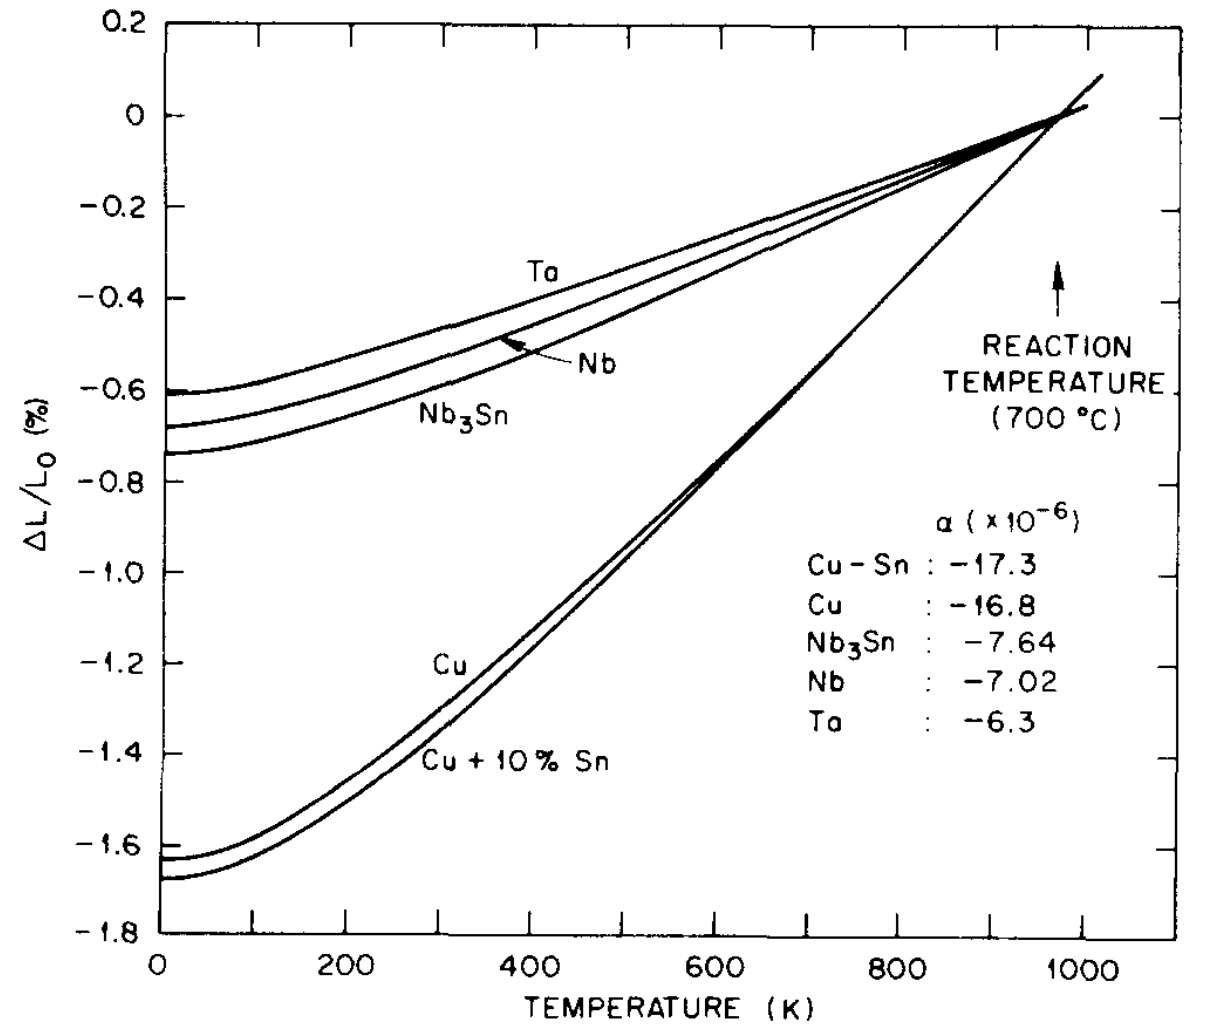
\includegraphics[width=0.6\textwidth]{images/intro/Nb3SnProperties/CTECuNbNb3Sn.png}
    \caption{Thermal expansion of Cu, Nb, and Nb$_3$Sn relative to \qty{700}{\degreeCelsius}~\cite{eastonPredictionStressState1980}. The Cu-Nb$_3$Sn mismatch is large; the Nb-Nb$_3$Sn mismatch is small, making Nb the ideal strain-free reference substrate.}
    \label{fig:CTECuNbNb3Sn}
\end{figure}


\section{Experimental detail}

\subsection{Substrate preparation and Cu-Sn deposition}

Niobium (1\,mm thick, high purity), c-plane sapphire, and oxygen-free high-conductivity (OFHC) copper substrates were cut into \qtyproduct{7.5 x 7.5}{\milli\meter} coupons and polished to a mirror finish using progressive SiC paper (400--1200 grit), diamond slurry (5--\qty{1}{\micro\meter}), and vibratory colloidal silica (\qty{0.05}{\micro\meter}). All substrates were ultrasonically cleaned in acetone and isopropyl alcohol before deposition. For Cu substrates, a 500\,nm Ta diffusion barrier was DC-magnetron sputtered at \qty{200}{\degreeCelsius} (\qty{10}{\milli\torr} Ar, base pressure $\sim 5 \times 10^{-9}$\,Torr) before Cu-Sn deposition.

Cu-Sn source alloys were prepared by mixing Cu (99.9\% purity) and Sn (99.8\% purity) spherical powders (Alfa Aesar) at compositions of 7, 14, 21, and 26\,at.\%\,Sn, loaded into alumina-coated tungsten baskets. Films were thermally evaporated to target thicknesses of 2--5\,\unit{\um} in steps of \qty{1}{\micro\meter} with 30-minute cooling intervals between steps to limit peeling, at a base pressure of $\sim 3 \times 10^{-7}$\,Torr. The evaporated film composition measured by EDS after deposition differed from the source composition due to differential vapor pressures of Cu and Sn, and is reported as the deposited Sn concentration throughout.

\subsection{Nb deposition and Nb$_3$Sn reaction}

Following a 10-minute preheat at \qty{110}{\degreeCelsius} in the sputtering chamber load lock, Nb was deposited from a 2-inch magnetron gun (250\,W, 8\,mTorr Ar). Three reaction variants were used:

\begin{itemize}
    \item \textbf{Post-reaction}: Nb deposited at \qty{200}{\degreeCelsius}, then heated in the same chamber to 650--750\,\unit{\degreeCelsius} for 12 or 24\,hours. For long anneals, an argon tube furnace (UHP Ar, $4 \times 10^{-5}$\,Torr pre-evacuation) was used.
    \item \textbf{Hot-bronze}: Nb deposited directly onto a Cu-Sn surface pre-heated to $\sim$\qty{715}{\degreeCelsius}, forming Nb$_3$Sn in situ during deposition.
    \item \textbf{Hot-bronze + post-reaction}: Hot-bronze deposition followed by continued \qty{715}{\degreeCelsius} anneal for 1--3\,hours.
\end{itemize}

\subsection{Critical temperature and microstructural characterization}

Critical temperature was measured by SQUID magnetometry (Quantum Design MPMS-5) using zero-field-cooled (ZFC) protocol: cool to \qty{4}{\kelvin}, apply \qty{1}{\milli\tesla} parallel to the film, record magnetic moment in \qty{0.1}{\kelvin} steps to \qty{20}{\kelvin}. $T_c$ onset is defined as the highest temperature at which the normalized moment deviates from zero; $\Delta T_c$ spans 90\%--10\% of the transition. Cross-sectional microstructure was characterized by FIB-SEM (FEI Helios G4 UC) with EDS (Oxford X-MaxN) for elemental mapping and linescans.


\section{Results}

\subsection{Sapphire substrate: isolating the Cu-Sn layer strain contribution}

Sapphire (c-plane) has a CTE close to that of Nb$_3$Sn, making it a near-zero-strain substrate~\cite{eastonPredictionStressState1980}. A \qty{2}{\micro\meter} Cu-13\,at.\%\,Sn film was deposited on sapphire, followed by \qty{500}{\nano\meter} Nb sputtered at \qty{680}{\degreeCelsius}. Three successive states of the same sample were measured by SQUID (Fig.~\ref{fig:SapphireStrain}):

\begin{enumerate}
    \item \textbf{On sapphire}: $T_c = \qty{17.1}{\kelvin}$, sharp transition.
    \item \textbf{Peeled from sapphire} (Cu-Sn/Nb$_3$Sn bilayer free-standing): $T_c$ drops to \qty{16.8}{\kelvin}. The sapphire had partially compensated the compressive CTE strain from the Cu-Sn layer; removing it exposes the full Cu-Sn strain on Nb$_3$Sn.
    \item \textbf{Etched} (Cu-Sn removed with APS): $T_c$ rises to $\sim$\qty{17.6}{\kelvin} and a Nb transition appears. The Nb transition reveals that the Cu-Sn layer had magnetically screened unreacted Nb and Sn-poor Nb$_3$Sn from the SQUID measurement, indicating hidden inhomogeneity. The Cu-Sn residual layer alone suppresses $T_c$ by $\sim$\qty{1}{\kelvin} via CTE-induced compressive strain.
\end{enumerate}

\begin{figure}[htb]
    \centering
    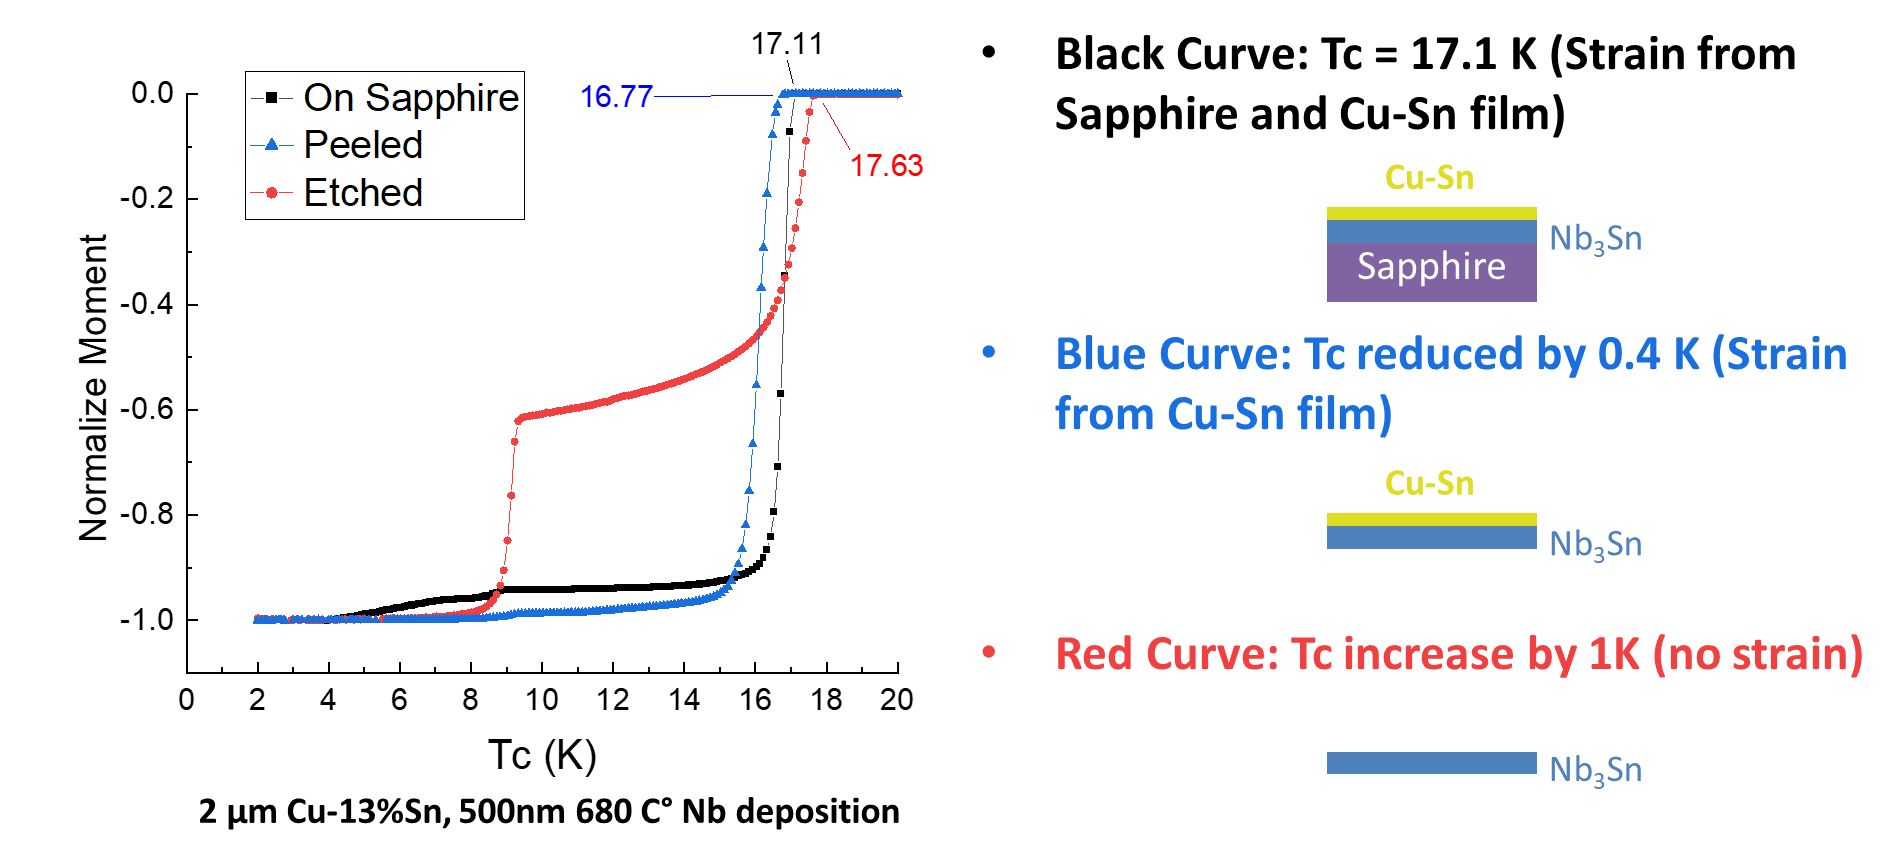
\includegraphics[width=0.85\textwidth]{images/Sapphire/SapphireStrain.png}
    \caption{$T_c$ curves for a hot-bronze film on sapphire: as-deposited on sapphire (black), peeled free-standing (blue), and etched to remove Cu-Sn (red). The Nb transition appearing after etching reveals previously screened unreacted Nb.}
    \label{fig:SapphireStrain}
\end{figure}

\subsection{Substrate comparison: mapping CTE strain to $T_c$ suppression}

To map CTE mismatch directly to $T_c$, the same recipe --- \qty{2}{\micro\meter} Cu-13\,at.\%\,Sn, \qty{500}{\nano\meter} Nb at \qty{680}{\degreeCelsius}, no pre/post treatment --- was applied to four substrates with identical conditions (Fig.~\ref{fig:SubstrateExpTc}):

\begin{itemize}
    \item \textbf{Sapphire}: $T_c \approx \qty{17}{\kelvin}$, sharp transition. Low CTE mismatch, sufficient Sn.
    \item \textbf{Nb}: $T_c \approx \qty{15}{\kelvin}$. Nb CTE matches Nb$_3$Sn, so the reduction is attributed to Sn depletion: the Nb substrate itself competes for Sn during reaction, leaving less Sn for the deposited Nb$_3$Sn layer.
    \item \textbf{Cu + Ta barrier}: $T_c \approx \qty{12}{\kelvin}$, broad transition. Large Cu CTE mismatch adds compressive strain; residual Sn depletion through Ta barrier.
    \item \textbf{Cu, no barrier}: $T_c \approx \qty{10}{\kelvin}$. Sn lost to Cu sink and maximum CTE strain combined.
\end{itemize}

\begin{figure}[htb]
    \centering
    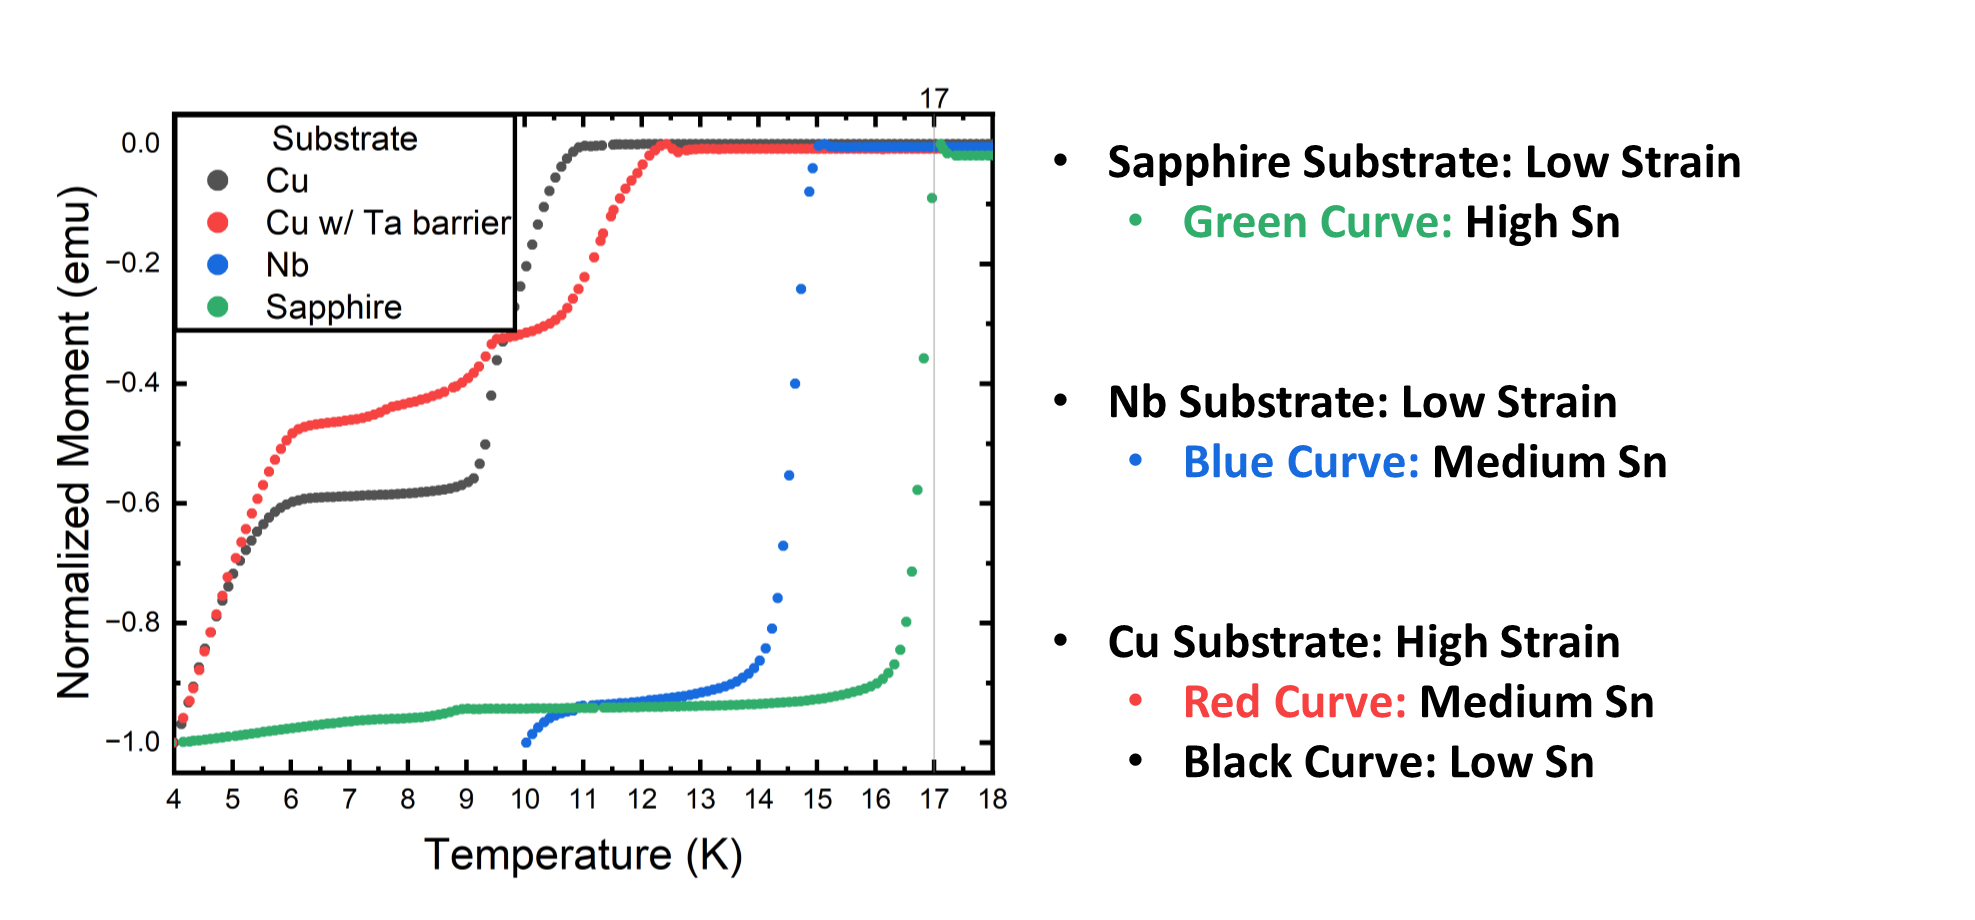
\includegraphics[width=0.9\textwidth]{images/Nb3Sn/SubstrateExpTc.png}
    \caption{$T_c$ curves for the same recipe on four substrates, demonstrating progressive CTE-strain and Sn-depletion suppression from sapphire (lowest impact) to Cu without diffusion barrier (highest impact).}
    \label{fig:SubstrateExpTc}
\end{figure}

\subsection{Nb substrate: optimal Sn concentration and reaction temperature}

The independence of strain on Nb substrates allows $T_c$ to serve as a direct measure of Sn content. A 30-sample matrix was prepared with five deposited Cu-Sn compositions (4, 13, 19, 33, 37\,at.\%\,Sn) at three reaction temperatures (650, 700, 750\,\unit{\degreeCelsius}) and two times (12, 24\,hr), reacted in a positive-pressure Ar tube furnace. Results are summarized in Fig.~\ref{fig:NbSubTcandSChem}.

Higher temperature consistently increased $T_c$, consistent with increased Sn diffusion rate~\cite{godekeReviewPropertiesNb3Sn2006}. The 24-hour reaction produced a thicker Nb$_3$Sn layer but negligible $T_c$ improvement over 12 hours. The optimal deposited Cu-Sn composition was 30--46\,wt.\%\,Sn (19--33\,at.\%\,Sn as deposited). Below this range, insufficient Sn volume yielded Sn-depleted Nb$_3$Sn; above it, rough Cu-Sn morphology introduced spatial non-uniformity, broadening the transition. The maximum achieved $T_c = \qty{17.8}{\kelvin}$ was obtained at \qty{750}{\degreeCelsius} with 33\,wt.\%\,Sn (Fig.~\ref{fig:NbSubUpdated}).

\begin{figure}[htb]
    \centering
    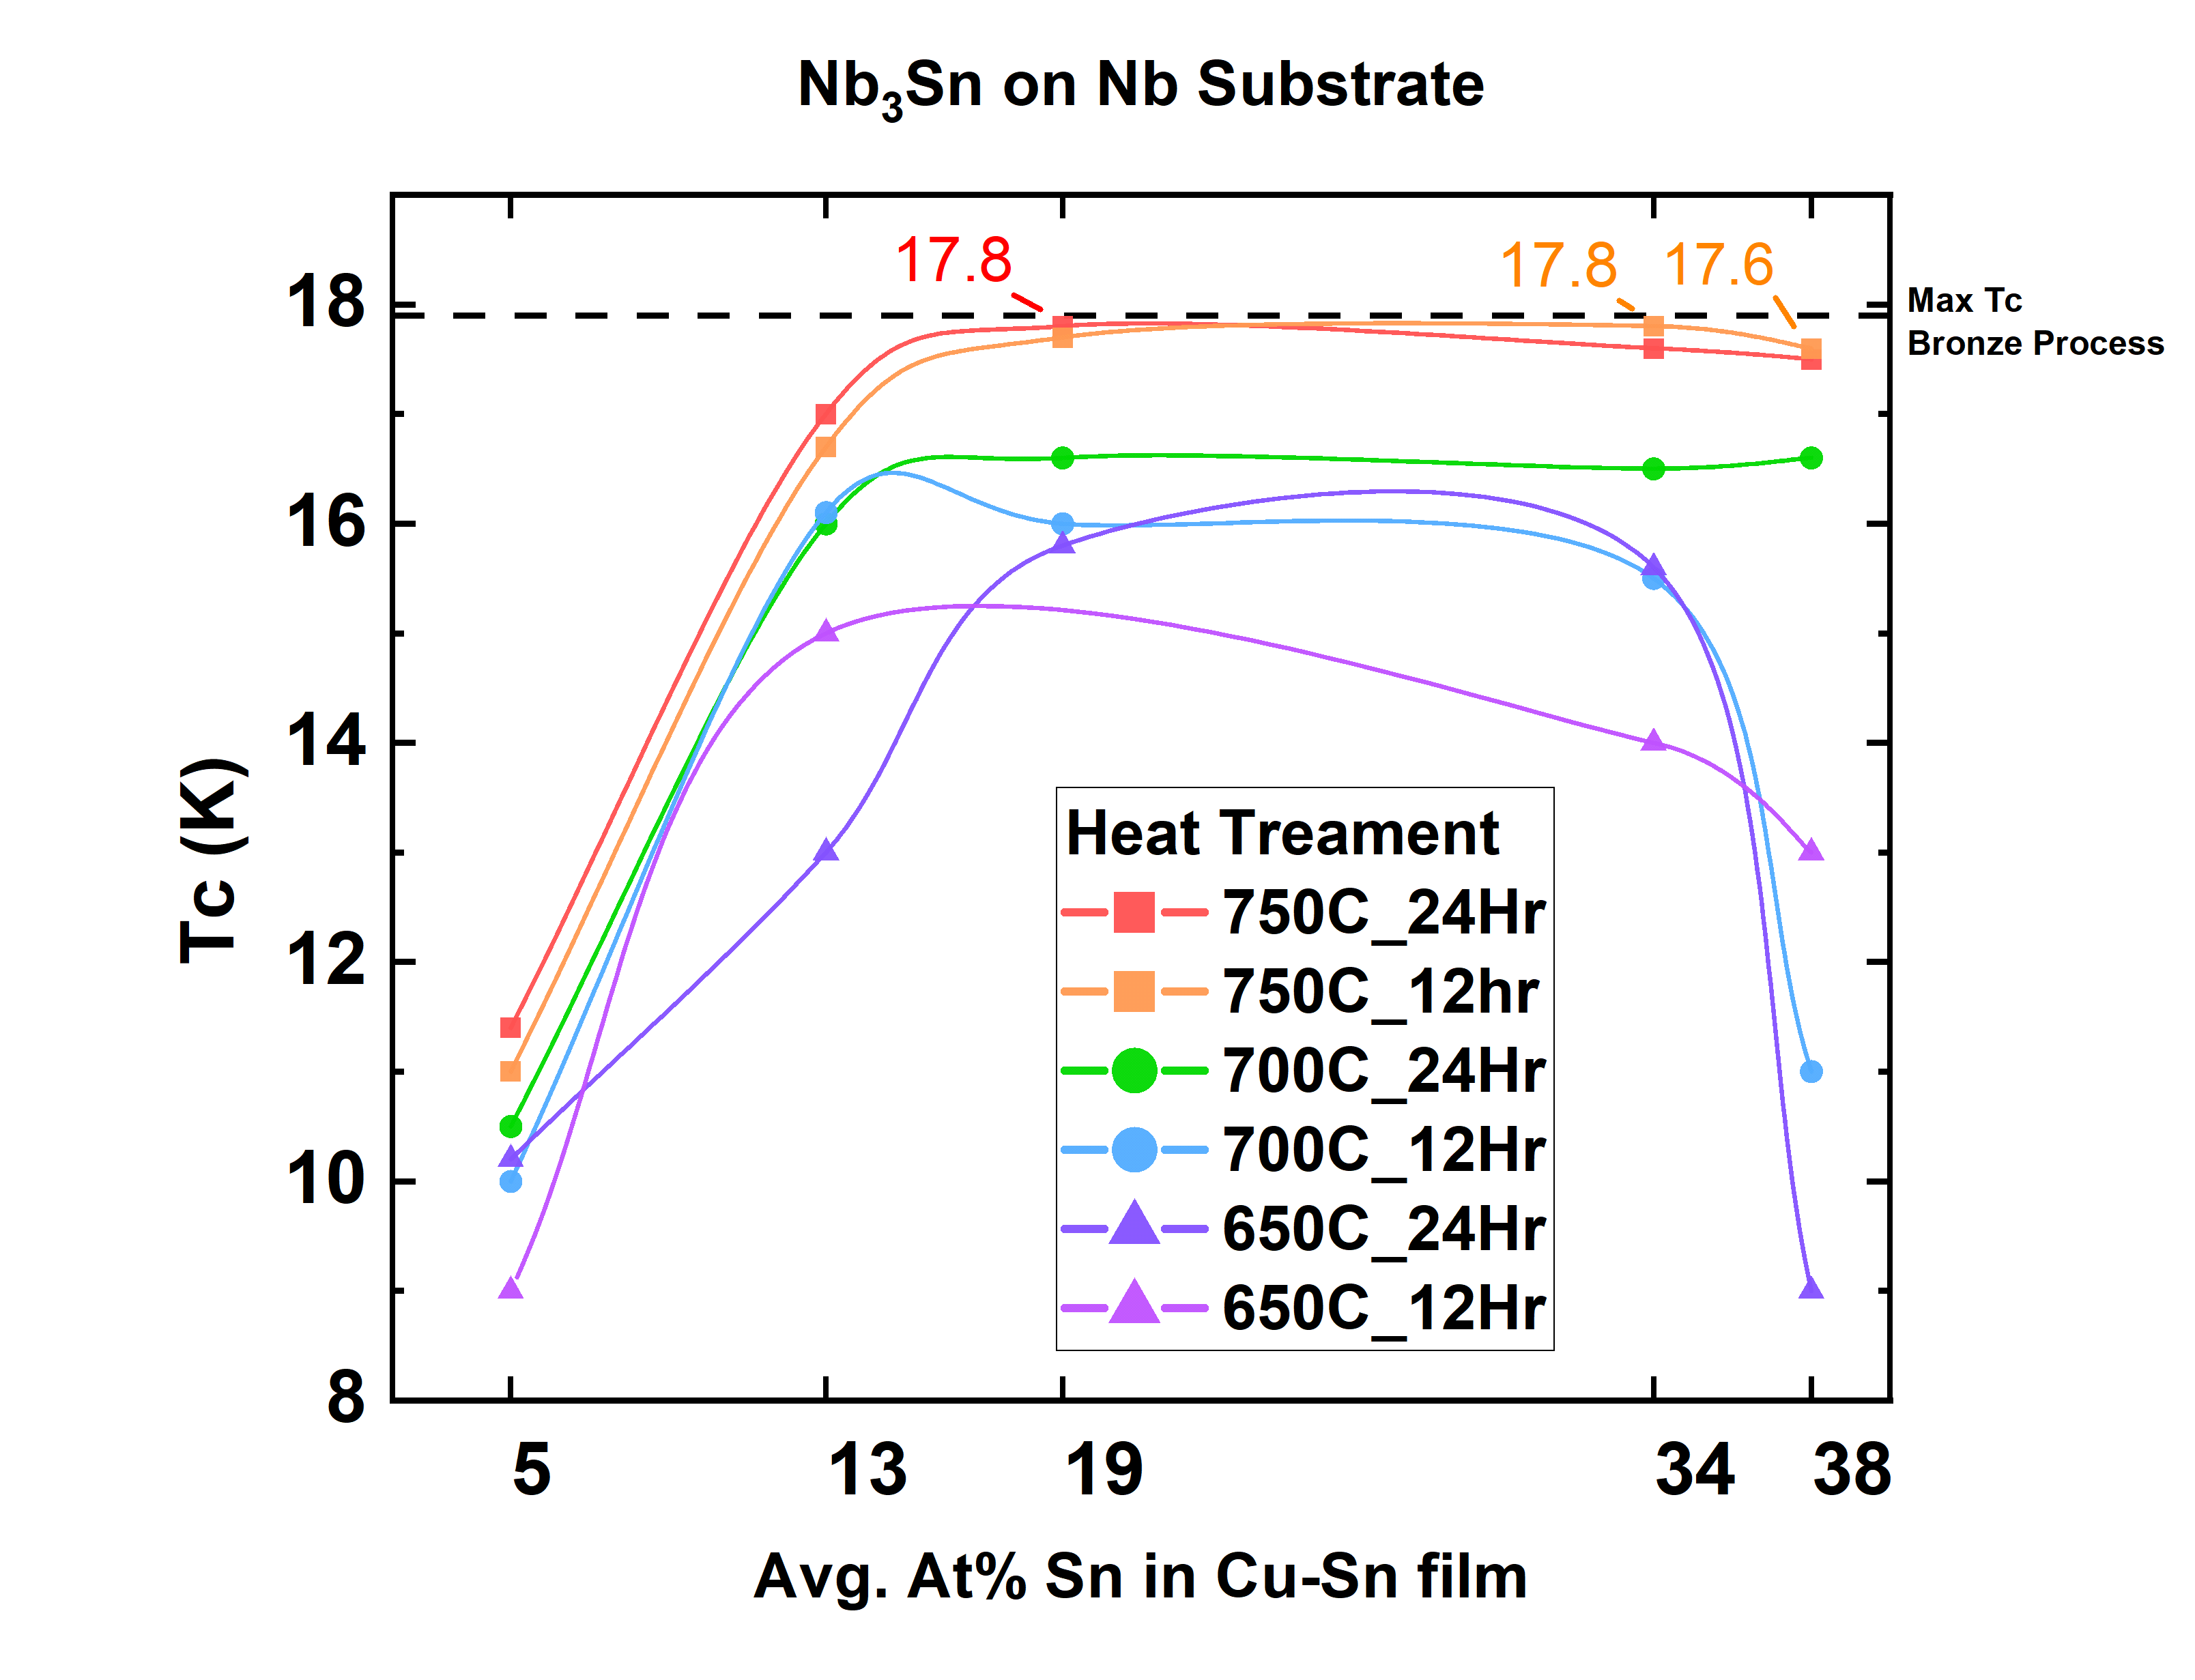
\includegraphics[width=0.85\textwidth]{images/Nb/NbSubUpdated.png}
    \caption{$T_c$ onset vs. deposited Cu-Sn Sn content for Nb-substrate samples reacted at 650, 700, and \qty{750}{\degreeCelsius} for 12 and 24\,hr. Maximum $T_c = \qty{17.8}{\kelvin}$ at \qty{750}{\degreeCelsius} with 33\,wt.\%\,Sn.}
    \label{fig:NbSubUpdated}
\end{figure}

\begin{figure}[htb]
    \centering
    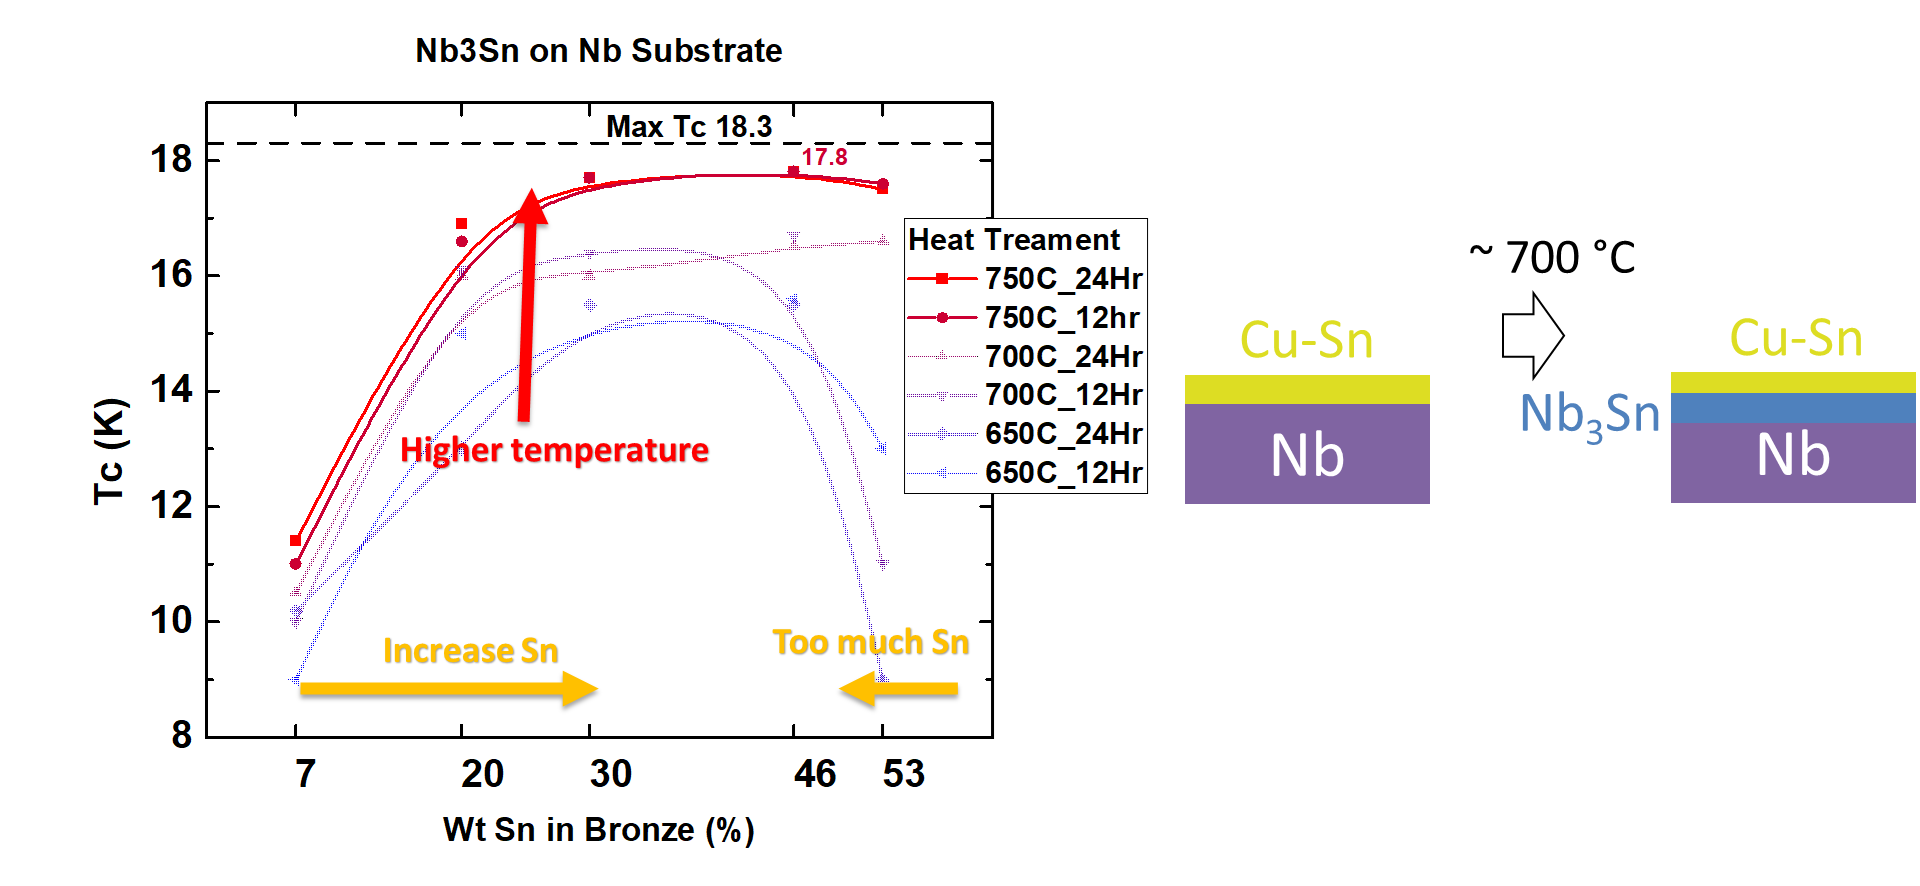
\includegraphics[width=0.85\textwidth]{images/Nb/NbSubTcandSChem.png}
    \caption{Full $T_c$ transition curves for Nb-substrate samples at all Sn concentrations and heat-treatment profiles. Each curve represents one sample from the 30-sample matrix.}
    \label{fig:NbSubTcandSChem}
\end{figure}

EDS linescans (Fig.~\ref{fig:linescan25Sn}) confirm that the best films contain $\sim$25\,at.\%\,Sn uniformly distributed across the Nb$_3$Sn thickness, consistent with stoichiometric Nb$_3$Sn~\cite{mooreEnergyGaps151979}.

\begin{figure}[htb]
    \centering
    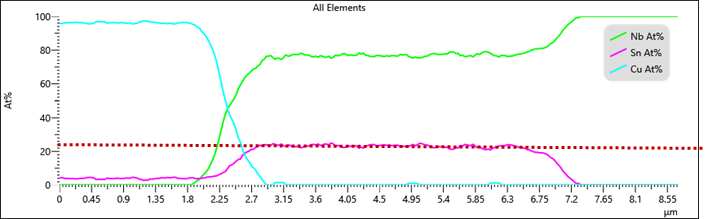
\includegraphics[width=0.8\textwidth]{images/Cu/linescan25Sn.png}
    \caption{EDS linescan across a hot-bronze Nb$_3$Sn film on a Nb substrate confirming $\sim$25\,at.\%\,Sn uniformly distributed through the film thickness.}
    \label{fig:linescan25Sn}
\end{figure}

\subsection{Hot-bronze on Nb substrates}

The hot-bronze technique was applied to Nb substrates by pre-heating to \qty{715}{\degreeCelsius} and depositing a \qty{3}{\micro\meter} Cu-Sn/Nb bilayer. The hot-bronze reaction formed Nb$_3$Sn simultaneously on both the top surface (from incoming Nb atoms reacting with hot Cu-Sn) and at the substrate interface (solid-state diffusion of Sn into the Nb substrate). Cross-sectional FIB-SEM/EDS (Fig.~\ref{fig:NbHot}) shows two distinct Nb$_3$Sn layers separated by the residual Cu-Sn film. The hot-bronze film on top grew significantly faster than the diffusion-limited film below. This sample achieved $T_c = \qty{17.9}{\kelvin}$ with a sharp transition (Fig.~\ref{fig:Nb3SnonNbBest}), the highest $T_c$ obtained in this work.

\begin{figure}[htb]
    \centering
    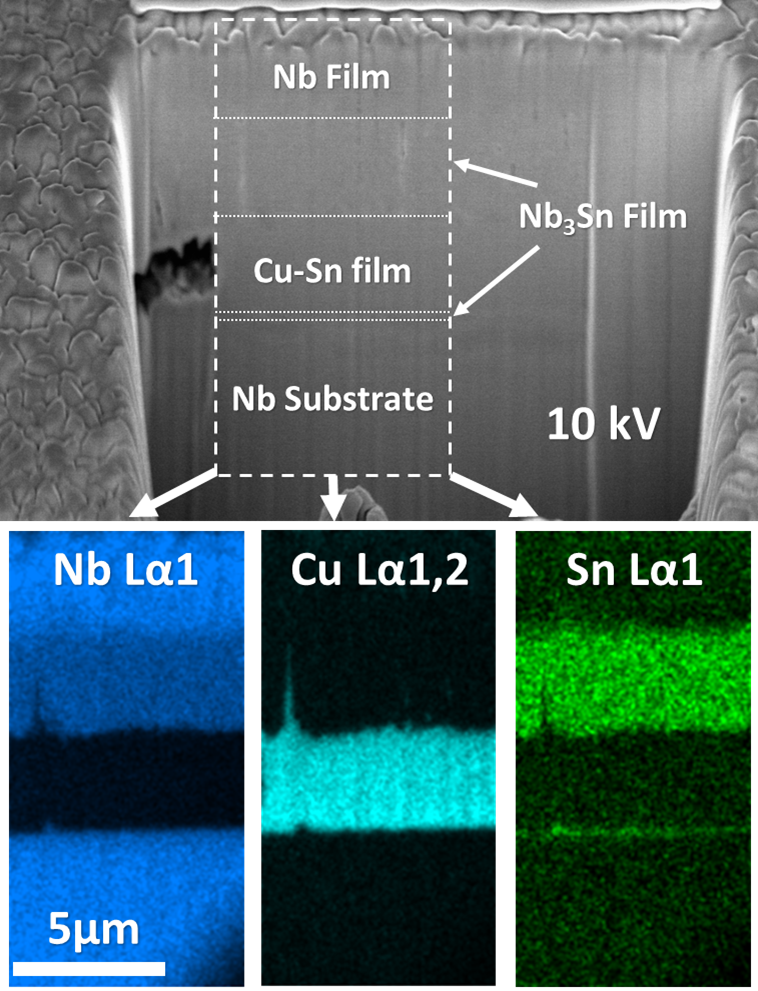
\includegraphics[width=0.6\textwidth]{images/Nb/NbHot.png}
    \caption{FIB cross-section SEM/EDS showing two Nb$_3$Sn layers on a Nb substrate: the upper layer formed by hot-bronze sputtering; the lower layer by solid-state diffusion into the Nb substrate.}
    \label{fig:NbHot}
\end{figure}

\begin{figure}[htb]
    \centering
    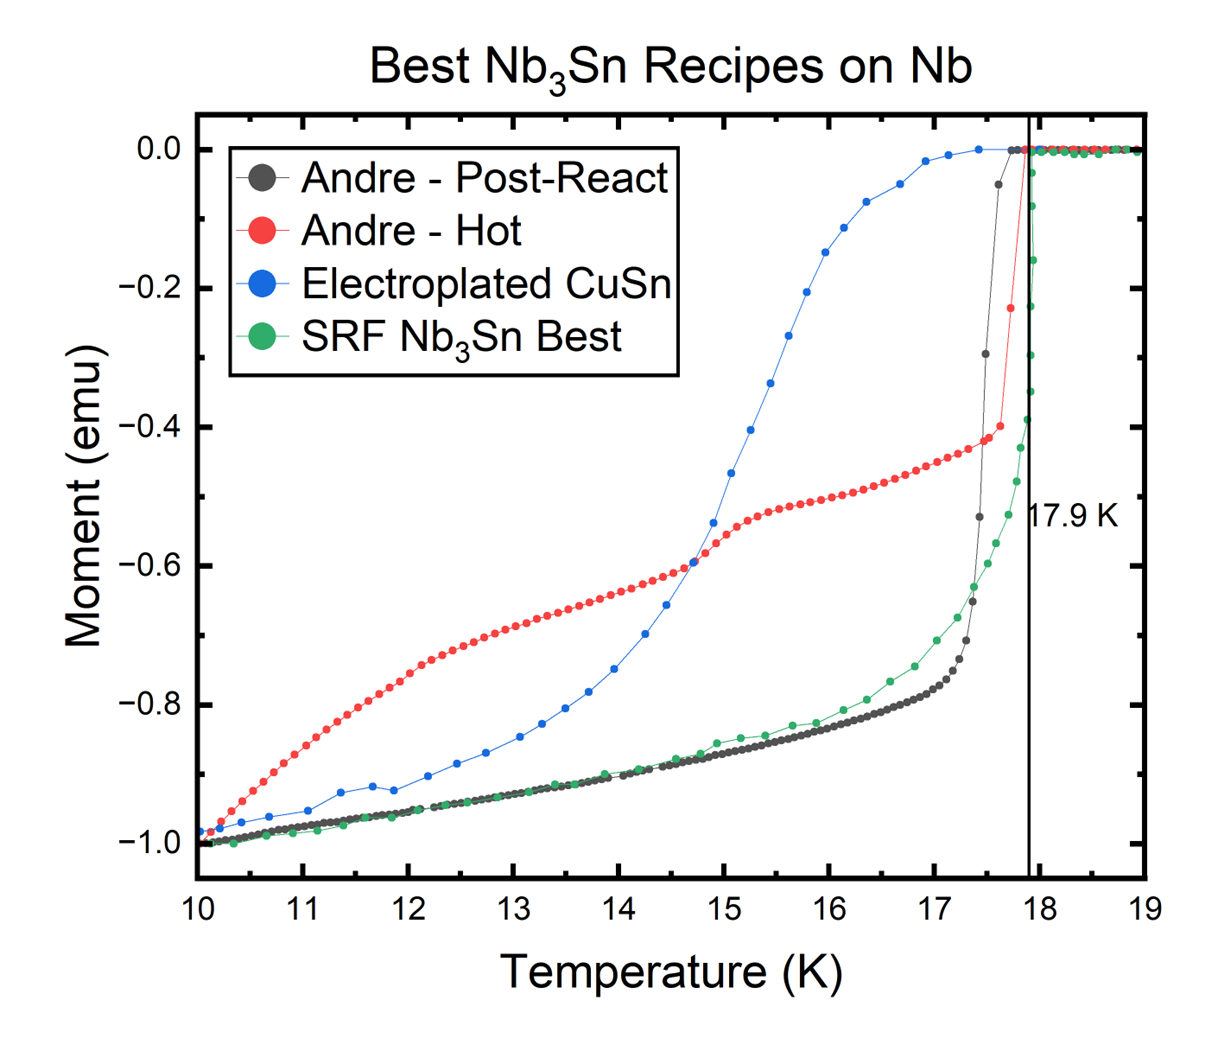
\includegraphics[width=0.6\textwidth]{images/Nb/Nb3SnonNbBest.png}
    \caption{$T_c$ curves comparing the best post-reacted and hot-bronze Nb-substrate films from this work with leading results from Sn vapor and electrochemical bronze routes. The hot-bronze film achieves $T_c = \qty{17.9}{\kelvin}$.}
    \label{fig:Nb3SnonNbBest}
\end{figure}

\subsection{Nb-first geometry and etching}

To address the Sn-surface vs. RF-surface trade-off on Cu substrates, the Nb-first geometry was demonstrated on Nb substrates: Cu-Sn was deposited on top of Nb and post-reacted, placing the Sn-rich Nb$_3$Sn nearest to the eventual RF surface after etching. Following post-reaction at \qty{715}{\degreeCelsius}, the Cu-Sn overlayer was selectively removed by ammonium persulfate (APS) etching. One half of the coupon was masked during etching to allow a direct cross-sectional comparison of etched and non-etched regions (Fig.~\ref{fig:NbsubetchSEM}). Both sides show continuous Nb$_3$Sn, confirming that APS etching selectively removes Cu-Sn without damaging the Nb$_3$Sn layer.

\begin{figure}[htb]
    \centering
    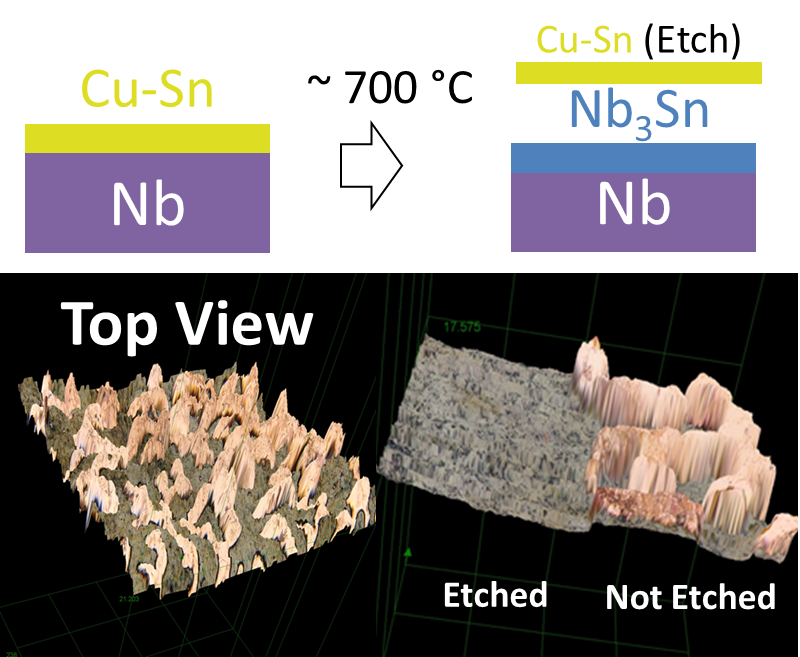
\includegraphics[width=0.9\textwidth]{images/Nb/Nbsubetching.png}
    \caption{Schematic and 3-D optical micrograph showing the Nb$_3$Sn film before and after APS etching to remove the Cu-Sn overlayer.}
    \label{fig:Nbsubetching}
\end{figure}

\begin{figure}[htb]
    \centering
    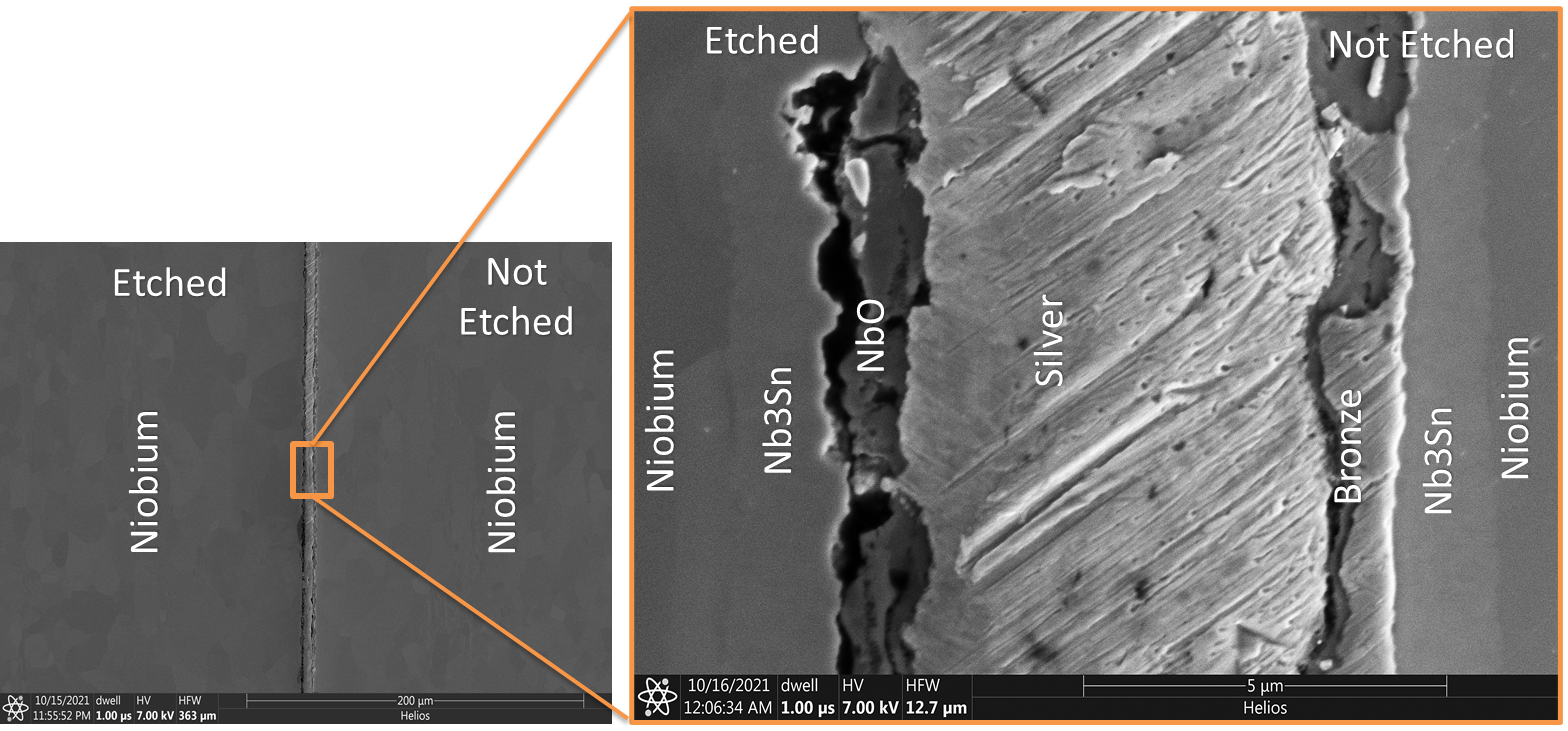
\includegraphics[width=0.9\textwidth]{images/Nb/NbsubetchSEM.png}
    \caption{Cross-sectional SEM of a Nb$_3$Sn film on Nb substrate: one half etched (left), one half non-etched (right), sandwiched together for direct comparison. Continuous Nb$_3$Sn is confirmed on both sides.}
    \label{fig:NbsubetchSEM}
\end{figure}


\section{Discussion}

The sapphire experiment establishes that the residual Cu-Sn layer beneath Nb$_3$Sn contributes $\sim$\qty{1}{\kelvin} of $T_c$ suppression via CTE-induced compression, independent of substrate. This is an intrinsic penalty of the Cu-Sn route regardless of substrate material and must be accounted for when interpreting measured $T_c$ values. On Nb substrates, the absence of bulk CTE mismatch isolates Sn content as the sole variable, enabling clean optimization: 33\,wt.\%\,Sn at \qty{750}{\degreeCelsius} achieves $T_c = \qty{17.8}{\kelvin}$, within \qty{0.5}{\kelvin} of the theoretical maximum.

The substrate comparison demonstrates quantitatively how each substrate contributes to $T_c$ suppression. The \qty{2}{\kelvin} gap between Nb and Cu substrates (both with optimal Sn) is dominated by CTE mismatch, not Sn depletion: on Cu, compressive strain at 4\,K lowers $T_c$ by $\sim$2\,K regardless of film stoichiometry~\cite{ekinStrainScalingLaw1980}. This explains why Recipe 2 (thick Nb$_3$Sn on Cu, \cite{Juliao2026}) achieved $T_c = \qty{17.7}{\kelvin}$ --- film thickness-dependent strain relaxation, not exceptional Sn stoichiometry. The hot-bronze Nb-substrate result ($T_c = \qty{17.9}{\kelvin}$, Fig.~\ref{fig:Nb3SnonNbBest}) is competitive with the best results from electrochemical bronze and Sn-vapor routes, validating the thermal evaporation Cu-Sn approach.

The Nb-first etching route establishes that APS selectively removes Cu-Sn without degrading Nb$_3$Sn, confirming its viability as a processing step for Cu-substrate cavities where the Cu-Sn overlayer must be removed after reaction. This is a prerequisite for applying the Nb-first recipe to RF cavity surfaces.


\section{Conclusions}

Systematic experiments on Nb and sapphire substrates established the fundamental limits of the Cu-Sn thin-film Nb$_3$Sn process independent of substrate CTE effects. The key findings are:

\begin{enumerate}
    \item The residual Cu-Sn layer suppresses $T_c$ by $\sim$\qty{1}{\kelvin} via compressive strain, independent of the substrate.
    \item CTE mismatch between substrate and Nb$_3$Sn progressively reduces $T_c$ from \qty{17}{\kelvin} (sapphire) to \qty{10}{\kelvin} (Cu, no barrier), with Nb substrates showing only \qty{2}{\kelvin} depression due to Sn competition.
    \item The optimal Cu-Sn deposited composition for Nb substrates is 30--46\,wt.\%\,Sn, yielding $T_c = \qty{17.8}{\kelvin}$ at \qty{750}{\degreeCelsius} and $T_c = \qty{17.9}{\kelvin}$ with hot-bronze deposition.
    \item APS etching selectively removes Cu-Sn without degrading Nb$_3$Sn, enabling the Nb-first RF cavity route.
\end{enumerate}

These results set the stoichiometric and microstructural baseline for optimizing Nb$_3$Sn on copper substrates, where CTE strain is the dominant performance limiter.

\ack
Work at the Applied Superconductivity Center was supported by [funding source TBD]. The authors acknowledge the NHMFL user program for instrument access.

\section*{Data availability statement}
Data supporting this study are available from the corresponding author upon reasonable request.

\printbibliography

\end{document}
